\newpage
\section{Business Intelligence Basics} \label{toc:grundlagenbusinessintelligence}

This chapter lays the foundations for understanding \ac{BI}. Consequently, the reader should be able to understand the
\ac{BI} process in order to understand the explanations in later parts of the thesis. In order to achieve this,
the \ac{BI} process itself is explained in chapter \ref{toc:prozess}. process itself is explained. The following subchapters will focus on the
strategic added value of \ac{BI} and to what extent this can be measured. This becomes important for the last part of the thesis,
to understand why such a project might be worthwhile. Ultimately, chapter \ref{toc:einfuehrungsstrategien}
clarifies which prerequisites must be met from the operational side in order for an introduction of BI to be successful.

The term \ac{BI} originated in the 1990s and was first coined by Howard Dressner, an analyst with the Gartner Group.
[Cf.][p. 96]{watson2007current} Prior to this time, systems such as \ac{DSS} and \ac{EIS} were already in place to help management
to make decisions.\footcite[Cf.][p. 1]{foley2010business}\footcite[Cf.][p. 19]{niu2009cognition}
Since then, these static systems have evolved into dynamic systems, which fall under the term \ac{BI}
\footcite[Cf.][p. 26]{yeoh2010critical} There are many different definitions for \ac{BI}, each of which varies in subtleties
differ.\footcite[Cf.][p. 114]{muntean2013agile} A general and striking definition is provided by Eric Foley in his paper
"What is Business Intelligence?": "Business intelligence (BI) is a combination of processes, policies, culture, and
technologies for gathering, manipulating, storing, and analyzing data collected from internal and external sources, in order to
to communicate information, create knowledge, and inform decision making. BI helps report business performance, uncover new
business opportunities, and make better business decisions regarding competitors, suppliers, customers, financial issues,
strategic issues, products and services."\footcite[][p. 4]{foley2010business} It means that \ac{BI} is an environment,
in which data is collected to generate knowledge and decision support. It also provides the ability to determine
business and process inadequacies and to identify and analyze new business areas.
The possibility to carry out internal optimizations with the help of \ac{BI} is the central
property why \ac{BI} is considered for testing the hypotheses of this thesis.

\subsection{The Business Intelligence Process} \label{toc:prozess}

In order to realize a \ac{BI} process, a multitude of logical steps are needed, which together are seen as a process.
\footcite[Cf.][p. 3]{foley2010business} Figure \ref{figure:biprocessoverview} shows the basic structure of a \ac{BI} process.
Here, the first steps are more technical in nature. During the process this changes into steps
which are more characterized by business perspectives. Consequently, knowledge is
built out of data.\footcite[Cf.][p. 13]{kasemsap2016fundamentals}

\begin{figure}[H]
    \caption{The Business Intelligence Process}
    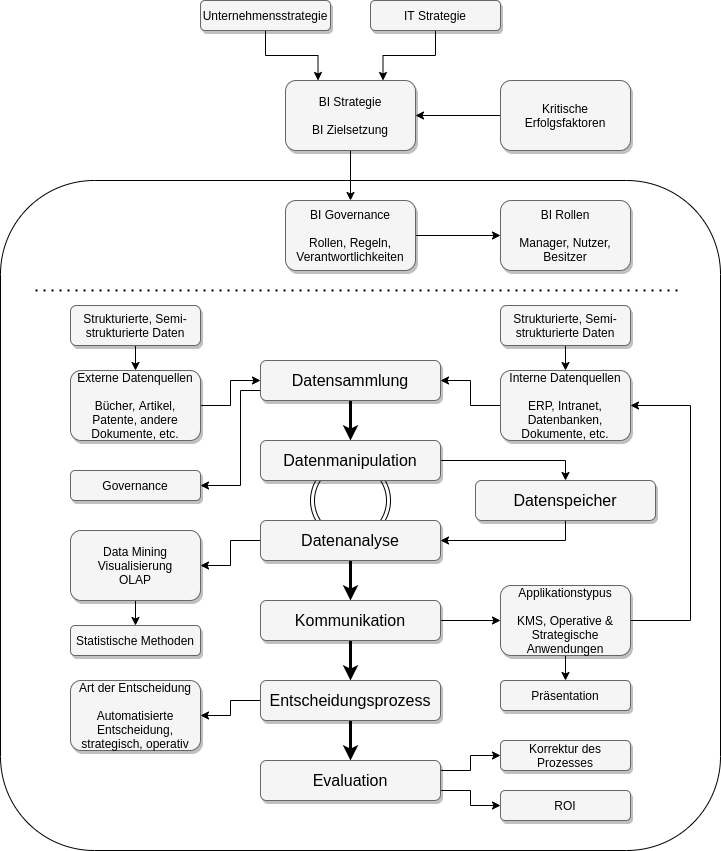
\includegraphics[width=0.7\textwidth]{biprocessoverview}
    \label{figure:biprocessoverview}
    \\
    \cite[Source: Based on][Fig. 2]{foley2010business}
\end{figure}

A \ac{BI} Process breaks down into six main activities:\footcite[Cf.][Fig. 2]{foley2010business}
\begin{itemize}
    \item \textbf{Data collection: }At the beginning all data is collected. This step is needed to execute the following
    process sections. Both internal and external data sources can be used. It does not have to be
    necessarily structured data. In principle, it can also be semi-structured and unstructured data.
    \footcite[Cf.][p. 465]{ranjan2008business}\footcite[Cf.][p. 3]{hartmann2016capturing}
    \item \textbf{Manipulation of data: }In this step, the collected data is structured in such a way that
    they can be stored in a \ac{DW}.\footcite[Cf.][p. 463]{ranjan2008business} The goal here is to have the most
    efficient data processing that takes into account the needs of the stakeholders and the users of this data.
    At the end of this step, the data is stored in a "Data Storage" (Cf. Fig. \ref{figure:biprocessoverview}).
    This is either a data warehouse or a data mart. The first two steps of the \ac{BI} process are therefore nothing else then a
    pipeline in which the data is queried, structured and stored in a \ac{DW}.
    \footcite[Cf.][p. 466]{ranjan2008business} Such a system can be realized for example by "Apache Hadoop" and
    "Spark".\footcite[Cf.][p. 65]{rahman2015big}
    \item \textbf{Analysis of the data: }The following step is an analysis of data that can be found in a data warehouse or similar
    system.\footcite[Cf.][p. 16]{kasemsap2016fundamentals}This can be achieved by a wide variety of systems
    and is very much tailored to the objective of the process.\footcite[Cf.][p. 21]{niu2009cognition} Therefore, it is important,
    that the requirements of the stakeholders are accurately implemented, so that no wrong analysis and results are presented and in the worst case,
    lead to completely wrong decisions. In this step, among other things, \ac{OLAP}
    systems are used, which allow multidimensional comparisons and analyses of the data.
    \footcite[Cf.][pp. 107]{hovcevar2010assessing} Other systems from the fields of machine learning and data mining are also used.
    \footcite[Cf.][p. 11]{foley2010business}\footcite[Cf.][p. 80]{yeoh2008managing} Additionally, the
    execution of simulations (for example, Monte Carlo simulations) is possible in this step. Finally, at the
    the result of the analyses and calculations, the management is provided with knowledge, which has an advantage over competitors, especially with respect to
    decision-making processes.\footcite[Cf.][p. 94]{hovcevar2010assessing}
    \item \textbf{Communication and Access: }Through the step of data analysis, it has been achieved that knowledge has been
    has been extracted from data. Making this knowledge accessible is the task of this step. The aim here is to ensure that the knowledge
    is made accessible to the right stakeholders via the right medium.\footcite[Cf.][p. 11]{foley2010business} These
    media can be dashboards, reports, scorecards and other methodologies.\footcite[Cf.][pp. 21]{niu2009cognition} At the end of
    of this step, the knowledge is accessible to stakeholders so that the next step can begin.
    \item \textbf{Decision Process: }In this step, the actual decision is made by the relevant stakeholder.
    \footcite[Cf.][p. 12]{foley2010business} In this process, the processed data are made available to support the
    decisions. This allows them to transparently base their decisions on the data collected.
    \footcite[Cf.][p. 13]{kasemsap2016fundamentals}
    \item \textbf{Evaluation: }The final step is to evaluate whether the \ac{BI} system brings the hoped-for improvements or benefits.
    On the one hand, it can be shown that the system is financially worthwhile and contributes to the success of the company.
    \footcite[Cf.][p. 12]{foley2010business} On the other hand, corrective measures can also be introduced in this step.
    measures can be introduced if the \ac{BI} Process did not bring the desired success.\footcite[Cf.][p. 12]{foley2010business}
    This approach gives the entire \ac{BI} process an agile and cyclical character.
\end{itemize}

As can be seen in figure \ref{figure:biprocessoverview}, there are other factors that contribute to a functioning
\ac{BI} Process. First and foremost, these include the strategy and goal definition of a \ac{BI} project. These are decisively
influenced by the \ac{CSF}. In chapter \ref{toc:einfuehrungsstrategien}, the factors are analyzed in more detail, as they have a
significant influence on a successful implementation. In addition, there is the issue of "IT governance".
In the case of \ac{BI}, this refers to the set of all guidelines and the bodies responsible for ensuring that the
areas of the project are clearly regulated.\footcite[Cf.][p. 8]{foley2010business} Finally, with the
the introduction of this governance the \ac{ROI} of the \ac{BI} Project.\footcite[Cf.][p. 8]{foley2010business}

\subsection{Added value for businesses} \label{toc:strategischermehrwert}

In IT projects, it is usually difficult to estimate the total added value for a company, which can be defined primarily by the
the \ac{ROI}.\footcite[Cf.][p. 97]{hovcevar2010assessing} This is due to the division of added value
into financial factors, which are comparatively easy to name, and into non-financial factors, which are indirectly measurable
and therefore can only be estimated.\footcite[Cf.][p. 93]{hovcevar2010assessing} This is true for \ac{BI} processes. Since an \ac{BI}
process has its central advantage in supporting management decision-making, and this can be very complex, the
financial impact may only be estimated.\footcite[Cf.][pp. 94]{hovcevar2010assessing} In figure
\ref{figure:mehrwertbi} are listed added values that an \ac{BI} Process can have for an organization. These are ranked in descending order
by the difficulty of measuring the financial value added.

\begin{figure}[H]
    \caption{Added value of Business Intelligence}
    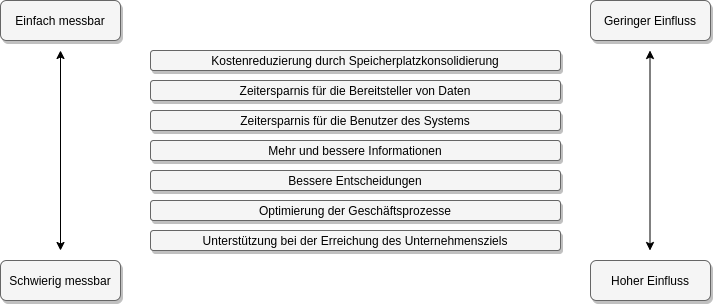
\includegraphics[width=0.85\textwidth]{mehrwertbi}
    \label{figure:mehrwertbi}
    \\
    \cite[Source: Based on][Fig. 2]{watson2007current}
\end{figure}

According to figure \ref{figure:mehrwertbi}, the added value of a BI process can be divided into the following areas:
\footcite[Cf.][Fig. 2]{watson2007current}

\begin{itemize}
    \item By introducing a data warehouse or a data mart, company-relevant data is stored in one place for analysis.
    Costs for a multitude of heterogeneous storage locations can be reduced. The availability
    of the data is improved. As a result, a reduction in costs is possible through a uniform system of data storage.
    \footcite[Cf.][p. 105]{azma2012business}
    \item Due to automated data procurement for the data warehouse and fast availability through \ac{OLAP} systems,
    a time saving in the process of data procurement and provision can also be measured.\footcite[Cf.][p. 51]{horakova2013business}
    This can be translated into a financial measure and considered in costs analysis.
    \item Since business-relevant data is stored in one place, making it quickly available to users,
    a time saving is measurable for the stakeholders of the system.\footcite[Cf.][p. 97]{williams2003business} As with the
    last point, this can also be added to the analysis.
    \item As one of the results of the BI process, information and knowledge are available more quickly. The quality of the
    information is higher than before because the information is based on larger amounts of data, more data sources and better analysis
    parameters\footcite[Cf.][p. 51]{horakova2013business}. Parameters such as information quality are factors,
    that can only enter into a financial analysis by estimation.\footcite[Cf.][p. 51]{horakova2013business}
    \item As a consequence of the better information situation, management is now in a position to make decisions better
    decisions. As described at the beginning, such a decision can be measured poorly in financial terms due to the high complexity and the large impact of the decision.
    \footcite[Cf.][p. 51]{horakova2013business} In addition, the opportunity costs are difficult to measure.
    \footcite[Cf.][p. 99]{hovcevar2010assessing}
    \item Business processes can be optimized using \ac{BI}. This is due to the better information situation and
    thus the possibility to identify inadequacies. The advantage obtained in this way is a difficult
    difficult to assess, as it is not possible to predict in advance to what extent process optimization will be necessary and what the financial impact will be.
    \footcite[Cf.][p. 2]{williams2003business}
    \item One of the foundations for the introduction of \ac{BI} is a clear business objective (see chapter \ref{toc:einfuehrungsstrategien}).
    \ac{BI} can help to achieve this faster and better. However, since many more factors than only one BI process
    contribute to the achievement of the business goal, it is difficult to identify the rightful share and to include it in the
    analysis of the added value.\footcite[Cf.][p. 51]{horakova2013business}
\end{itemize}

Im Gegensatz zu dem Mehrwert sind die Kosten für ein \ac{BI} Projekt recht einfach abschätzbar, indem diese für die Infrastruktur,
Software und das Projektteam in Betracht gezogen werden.\footcite[Cf.][p. 98]{hovcevar2010assessing} Die Kostenersparnisse
und Einnahmen durch einen \ac{BI} Prozess müssen die Ausgaben übersteigen, damit ein \ac{ROI} messbar
wird.\footcite[Cf.][p. 8]{williams2003business} Nur falls dies möglich ist, kann ein unternehmensweiter Mehrwert des Projekts
identifiziert werden und dadurch auch die Sinnhaftigkeit gegenüber dem Management dargelegt werden. Zusammenfassend ist
feststellbar, dass sich der hauptsächliche Mehrwert von BI folgendermaßen definieren lässt: "`the business value of BI lies in
its effective use within management processes and/or operational processes that drive revenue or reduce
costs."'\footcite[][p. 7]{williams2003business}

\subsection{Prerequisites for a successful introduction} \label{toc:einfuehrungsstrategien}

The prerequisites necessary for successful implementation are described in the critical success factors.

\begin{figure}[H]
    \caption{Prerequisites for a successful BI implementation}
    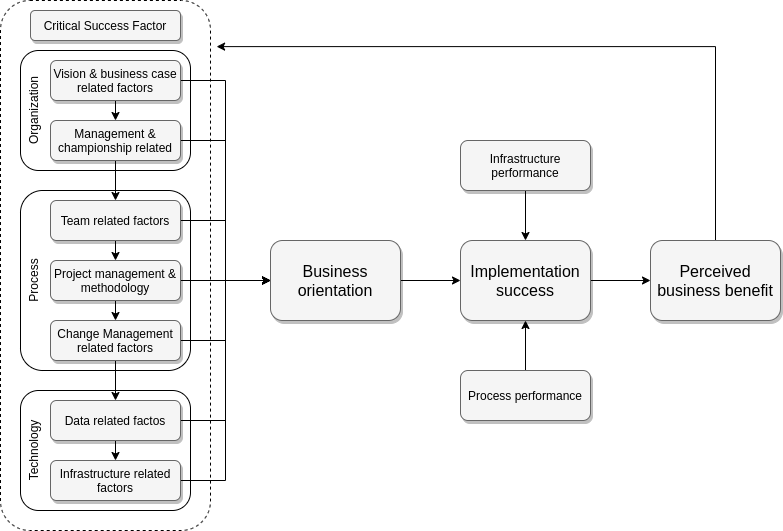
\includegraphics[width=0.85\textwidth]{bisuccessfactors}
    \label{figure:bisuccessfactors}
    \\
    \cite[Source: Based on][Fig. 1]{yeoh2010critical}
\end{figure}

In figure \ref{figure:bisuccessfactors}, these success factors are divided into three different dimensions and thus different
viewpoints.\footcite[Cf.][pp. 26]{yeoh2010critical} Using these dimensions, it is later possible to perform a
stakeholder analysis for a \ac{BI} process. The three different perspectives can be defined as follows:

\begin{itemize}
    \item \textbf{Organizational View: }This dimension is based on a view from the direction of the organization.
    There are two points that make the success of a \ac{BI} Process possible. The first point requires that the project
    receives clear support from management. This ensures that the project has sufficient financial and human resources.
    \footcite[Cf.][p. 98]{watson2007current} A project sponsor on the part of the management is recommended.
    \footcite[Cf.][pp. 87]{yeoh2008managing} The second point is that the project must have a clear objective and vision.\footcite[Cf.][pp. 87]{yeoh2008managing}
    \footcite[Cf.][p. 50]{villamarin2017key} This requires a company, that wants to implement such a process, to have a clear vision.
    Based on this, it is possible to formulate the project vision and ultimately define a clear
    objective for the project.\footcite[Cf.][pp. 87]{yeoh2008managing}
    \item \textbf{Process View: }This view looks at the actual processes and requirements at the project level.
    First and foremost, there is a project management team that is capable of managing the project. Such a project manager should have the
    technical, organizational, and process perspectives.\footcite[Cf.][p. 27]{yeoh2010critical}He must be as familiar with the
    processes in the company as well as with the characteristics of the technical systems used to solve the problem.
    \footcite[Cf.][pp. 88]{yeoh2008managing} In addition, a well-balanced team composition is very important.
    \footcite[Cf.][pp. 87]{yeoh2008managing} Since the implementation of BI processes is typically of an
    interdisciplinary nature, the team should consist of both specialists in technology and specialists in
    data analysis, data presentation, and business processes.\footcite[Cf.][Fig. 7]{muntean2013agile} Last but not least.
    a flexible and agile development approach is recommended, since \ac{BI} systems in particular should react quickly to changing requirements.
    Only through this flexibility is it possible to react quickly if something needs to be changed, improved
    or should be updated. One methodology to achieve this is
    Scrum.\footcite[Cf.][p. 164]{isik2011business}\footcite[Cf.][p. 3817]{knabke2013understanding}
    \item \textbf{Technological view: }Finally, the technological view is important. This is divided into two
    subject areas: On the one hand, there are the success factors that deal with the data
    \footcite[Cf.][Fig. 1]{yeoh2010critical} These factors primarily describe the nature of the data used.
    Two requirements are placed on the data: The data should be of both high quality and high
    integrity.\footcite[Cf.][p. 163]{isik2011business} Both could lead to distorted results,
    which could lead to an unusable BI system. On the other hand, there are factors that affect the infrastructural side.
    \footcite[Cf.][Fig. 1]{yeoh2010critical} Above all, the underlying infrastructure should be flexible and
    scalable. It must be able to respond to changing demands on the project.
    \footcite[Cf.][pp. 89]{yeoh2008managing}
\end{itemize}

On the basis of these critical success factors, it is possible to check during project planning whether the most important
prerequisites for a project implementation are given. Later in this work, such an analysis will be carried out concretely.